\documentclass[9pt,dvipsnames]{beamer}
\usepackage[T1]{fontenc}
\usepackage{libertinus}
\usepackage{amsmath}
\usepackage[most]{tcolorbox}

\usepackage{graphicx}

\usepackage{hyperref}
% \hypersetup{
%     colorlinks=true,
%     linkcolor=blue,    % color of internal links
%     urlcolor=blue,     % color of external URLs
%     citecolor=blue     % color of citations
% }

\usepackage{xcolor}  
\newcommand{\cb}[1]{{\color{CadetBlue}#1}}


\usetheme{Berkeley}
% \setbeamertemplate{footline}[frame number]
\setbeamertemplate{navigation symbols}{}


\title{CSE574 Introduction to Machine Learning}
\subtitle{Machine Learning: Notation and Definitions}
\author{Jue Guo}
\institute{University at Buffalo}
\date{\today}

\begin{document}
\begin{frame}
	\titlepage
\end{frame}

\begin{frame}
	\frametitle{Outline}
	\tableofcontents
\end{frame}

\section{Notation}
\begin{frame}{Notation}
	Let's breifly revisit the mathematical notation we all learned at school.
\end{frame}

\subsection{Data Structure}
\begin{frame}{Data Structure}
	A \textbf{scalar} is a simple numerical value, like 15 or -3.25 . Variables or constants that take scalar values are denoted by an italic letter, like $x$ or $a$.

	A \textbf{vector} is an ordered list of scalar values, called attributes. We denote a vector as a bold character, for example, $\mathbf{x}$ or $\mathbf{w}$.
	\begin{itemize}
		\item Vectors can be visualized as arrows that point to some directions as well as points in a multi-dimensional space.
	\end{itemize}
	Illustrations of three two-dimensional vectors, $\mathbf{a}=[2,3], \mathbf{b}=[-2,5]$, and $\mathbf{c}=[1,0]$ are given in the figure.
	\begin{figure}
		\centering
		
\includegraphics[width=0.7\textwidth]{imgs/notation_1}
		\caption{Three vectors visualized as directions and as points.}
		\label{fig:notation1}
	\end{figure}
\end{frame}

\begin{frame}
	We denote an attribute of a vector as an italic value with an index, like this: $w^{(j)}$ or $x^{(j)}$. The index $j$ denotes a specific \textbf{dimension} of the vector, the position of an attribute in the list. For instance, in the vector a shown in red in the figure, $a^{(1)}=2$ and $a^{(2)}=3$.
	\begin{figure}
		\centering
		
\includegraphics[width=0.7\textwidth]{imgs/notation_1}
		\caption{Three vectors visualized as directions and as points.}
	\end{figure}
	The notation $x^{(j)}$ should not be confused with the power operator, such as the 2 in $x^{2}$ (squared) or 3 in $x^{3}$ (cubed). If we want to apply a power operator, say square, to an indexed attribute of a vector, we write like this: $\left(x^{(j)}\right)^{2}$.

	A variable can have two or more indices, like this: $x_{i}^{(j)}$ or like this $x_{i, j}^{(k)}$. For example, in neural networks, we denote as $x_{l, u}^{(j)}$ the input feature $j$ of unit $u$ in layer $l$.
\end{frame}

\begin{frame}
	A \textbf{matrix} is a rectangular array of numbers arranged in rows and columns. Below is an example of a matrix with two rows and three columns,
	$$
		\left[\begin{array}{ccc}
				2  & 4  & -3 \\
				21 & -6 & -1
			\end{array}\right]
	$$

	Matrices are denoted with bold capital letters, such as \(\mathbf{A}\) or \(\mathbf{W}\).

	A \textbf{set} is an unordered collection of unique elements.
	\begin{itemize}
		\item We denote a set as a calligraphic capital character, for example, $\mathcal{S}$.
	\end{itemize}
	\textcolor{red}{A set of numbers can be finite (include a fixed amount of values).}
	\begin{itemize}
		\item  In this case, it is denoted using accolades, for example, $\{1,3,18,23,235\}$ or $\left\{x_{1}, x_{2}, x_{3}, x_{4}, \ldots, x_{n}\right\}$.
	\end{itemize}

	\textcolor{red}{A set can be infinite and include all values in some interval.}
	\begin{itemize}
		\item If a set includes all values between $a$ and $b$, including $a$ and $b$, it is denoted using brackets as $[a, b]$. If the set doesn't include the values $a$ and $b$, such a set is denoted using parentheses like this: $(a, b)$.
	\end{itemize}

	\begin{itemize}
		\item For example, the set $[0,1]$ includes such values as $0,0.0001,0.25,0.784,0.9995$, and 1.0. A special set denoted $\mathbb{R}$ includes all numbers from minus infinity to plus infinity.
	\end{itemize}

\end{frame}

\begin{frame}
	When an element $x$ belongs to a set $\mathcal{S}$, we write $x \in \mathcal{S}$.
	\begin{itemize}
		\item 	We can obtain a new set $\mathcal{S}_{3}$ as an \textbf{intersection} of two sets $\mathcal{S}_{1}$ and $\mathcal{S}_{2}$. In this case, we write $\mathcal{S}_{3} \leftarrow \mathcal{S}_{1} \cap \mathcal{S}_{2}$. For example $\{1,3,5,8\} \cap\{1,8,4\}$ gives the new set $\{1,8\}$.
		\item 	We can obtain a new set $\mathcal{S}_{3}$ as a \textbf{union} of two sets $\mathcal{S}_{1}$ and $\mathcal{S}_{2}$. In this case, we write $\mathcal{S}_{3} \leftarrow \mathcal{S}_{1} \cup \mathcal{S}_{2}$. For example $\{1,3,5,8\} \cup\{1,8,4\}$ gives the new set $\{1,3,4,5,8\}$.
	\end{itemize}
\end{frame}

\subsection{Capital Sigma Notation}
\begin{frame}{Capital Sigma Notation}
	The summation over a collection $\mathcal{X}=\left\{x_{1}, x_{2}, \ldots, x_{n-1}, x_{n}\right\}$ or over the attributes of a vector $\mathbf{x}=\left[x^{(1)}, x^{(2)}, \ldots, x^{(m-1)}, x^{(m)}\right]$ is denoted like this:
	\begin{equation*}
		\begin{aligned}
			 & \sum_{i=1}^{n} x_{i} \stackrel{\text { def }}{=} x_{1}+x_{2}+\ldots+x_{n-1}+x_{n}, \\ & \text { or else: } \sum_{j=1}^{m} x^{(j)} \stackrel{\text { def }}{=} x^{(1)}+x^{(2)}+\ldots+x^{(m-1)}+x^{(m)}
		\end{aligned}
	\end{equation*}
	The notation $\stackrel{\text { def }}{=}$ means "is defined as".
\end{frame}

\subsection{Capital Pi Notation}
\begin{frame}{Capital Pi Notation}
	A notation analogous to capital sigma is the capital pi notation. It denotes a product of elements in a collection or attributes of a vector:

	$$
		\prod_{i=1}^{n} x_{i} \stackrel{\text { def }}{=} x_{1} \cdot x_{2} \cdot \ldots \cdot x_{n-1} \cdot x_{n}
	$$

	where $a \cdot b$ means $a$ multiplied by $b$. Where possible, we omit $\cdot$ to simplify the notation, so $a b$ also means $a$ multiplied by $b$.
\end{frame}

\subsection{Operations on Sets}
\begin{frame}{Operations on Sets}
	A derived set creation operator looks like this: $\mathcal{S}^{\prime}\leftarrow\left\{x^{2} \mid x \in \mathcal{S}, x>3\right\}$.
	\begin{itemize}
		\item This notation means that we create a new set $\mathcal{S}^{\prime}$ by putting into it $x$ squared such that $x$ is in $\mathcal{S}$, and $x$ is greater than 3.
	\end{itemize}
	The cardinality operator $|\mathcal{S}|$ returns the number of elements in set $\mathcal{S}$.
\end{frame}

\subsection{Operations on Vectors}
\begin{frame}{Operations on Vectors}
	\begin{itemize}
		\item The sum of two vectors $\mathbf{x}+\mathbf{z}$ is defined as the vector $\left[x^{(1)}+z^{(1)}, x^{(2)}+z^{(2)}, \ldots, x^{(m)}+z^{(m)}\right]$.
		\item The difference of two vectors $\mathbf{x}-\mathbf{z}$ is defined as $\left[x^{(1)}-z^{(1)}, x^{(2)}-z^{(2)}, \ldots, x^{(m)}-z^{(m)}\right]$.
		\item A vector multiplied by a scalar is a vector. For example $\mathbf{x} c \stackrel{\text { def }}{=}\left[c x^{(1)}, c x^{(2)}, \ldots, c x^{(m)}\right]$.
		\item A dot-product of two vectors is a scalar.
		      \begin{itemize}
			      \item For example, $\mathbf{w} \mathbf{x} \stackrel{\text { def }}{=} \sum_{i=1}^{m} w^{(i)} x^{(i)}$. The dot-product is denoted as $\mathbf{w} \cdot \mathbf{x}$. The two vectors must be of the same dimensionality. Otherwise, the dot-product is undefined.
		      \end{itemize}
		\item The multiplication of a matrix $\mathbf{W}$ by a vector $\mathbf{x}$ results in another vector. Let our matrix be,
		      $$
			      \mathbf{W}=\left[\begin{array}{lll}
					      w^{(1,1)} & w^{(1,2)} & w^{(1,3)} \\
					      w^{(2,1)} & w^{(2,2)} & w^{(2,3)}
				      \end{array}\right]
		      $$
	\end{itemize}
\end{frame}

\begin{frame}
	When vectors participate in operations on matrices, a vector is by default represented as a matrix with one column. When the vector is on the right of the matrix, it remains a column vector. We can only multiply a matrix by vector if the vector has the same number of rows as the number of columns in the matrix. Let our vector be $\mathbf{x} \stackrel{\text { def }}{=}\left[x^{(1)}, x^{(2)}, x^{(3)}\right]$. Then $\mathbf{W} \mathbf{x}$ is a two-dimensional vector defined as,

	$$
		\begin{aligned}
			\mathbf{W} \mathbf{x} & =\left[\begin{array}{lll}
					                               w^{(1,1)} & w^{(1,2)} & w^{(1,3)} \\
					                               w^{(2,1)} & w^{(2,2)} & w^{(2,3)}
				                               \end{array}\right]\left[\begin{array}{l}
					                                                       x^{(1)} \\
					                                                       x^{(2)} \\
					                                                       x^{(3)}
				                                                       \end{array}\right]                                      \\
			                      & \stackrel{\text { def }}{=}\left[\begin{array}{l}
					                                                         w^{(1,1)} x^{(1)}+w^{(1,2)} x^{(2)}+w^{(1,3)} x^{(3)} \\
					                                                         w^{(2,1)} x^{(1)}+w^{(2,2)} x^{(2)}+w^{(2,3)} x^{(3)}
				                                                         \end{array}\right] \\
			                      & =\left[\begin{array}{l}
					                               \mathbf{w}^{(1)} \mathbf{x} \\
					                               \mathbf{w}^{(2)} \mathbf{x}
				                               \end{array}\right]
		\end{aligned}
	$$

	If our matrix had, say, five rows, the result of the product would be a five-dimensional vector.
\end{frame}

\begin{frame}
	When the vector is on the left side of the matrix in the multiplication, then it has to be \textbf{transposed} before we multiply it by the matrix. The transpose of the vector $\mathbf{x}$ denoted as $\mathbf{x}^{\top}$ makes a row vector out of a column vector. Let's say,

	$$
		\mathbf{x}=\left[\begin{array}{l}
				x^{(1)} \\
				x^{(2)}
			\end{array}\right], \text { then } \mathbf{x}^{\top} \stackrel{\text { def }}{=}\left[\begin{array}{ll}
				x^{(1)} & x^{(2)}
			\end{array}\right]
	$$

	The multiplication of the vector $\mathbf{x}$ by the matrix $\mathbf{W}$ is given by $\mathbf{x}^{\top} \mathbf{W}$,

	\begin{equation*}
		\begin{aligned}
			\mathbf{x}^{\top} \mathbf{W} & =\left[\begin{array}{ll}
					                                      x^{(1)} & x^{(2)}
				                                      \end{array}\right]\left[\begin{array}{lll}
					                                                              w^{(1,1)} & w^{(1,2)} & w^{(1,3)} \\
					                                                              w^{(2,1)} & w^{(2,2)} & w^{(2,3)}
				                                                              \end{array}\right]                                                        \\
			                             & \stackrel{\text { def }}{=}[w^{(1,1)} x^{(1)}+w^{(2,1)} x^{(2)}, w^{(1,2)} x^{(1)}+w^{(2,2)} x^{(2)}, w^{(1,3)} x^{(1)} \\
			                             & +w^{(2,3)} x^{(2)}]
		\end{aligned}
	\end{equation*}
	As you can see, we can only multiply a vector by a matrix if the vector has the same number of dimensions as the number of rows in the matrix.
\end{frame}

\subsection{Functions}
\begin{frame}{Functions}
	A \textbf{function} is a relation that associates each element $x$ of a set $\mathcal{X}$, the \textbf{domain} of the function, to a single element $y$ of another set $\mathcal{Y}$, the \textbf{codomain} of the function. A function usually has a name.
	\begin{itemize}
		\item 	If the function is called $f$, this relation is denoted $y=f(x)$ (read $f$ of $x$ ), the element $x$ is the argument or input of the function, and $y$ is the value of the function or the output. The symbol that is used for representing the input is the variable of the function (we often say that $f$ is a function of the variable $x$ ).
	\end{itemize}
\end{frame}

\begin{frame}
	We say that $f(x)$ has a \textbf{local minimum} at $x=c$ if $f(x) \geq f(c)$ for every $x$ in some open interval around $x=c$.
	\begin{itemize}
		\item An \textbf{interval} is a set of real numbers with the property that any number that lies between two numbers in the set is also included in the set. An open interval does not include its endpoints and is denoted using parentheses. For example, $(0,1)$ means "all numbers greater than 0 and less than 1 ".
	\end{itemize}
	The minimal value among all the local minima is called the \textbf{global minimum}.
	\begin{figure}
		\centering
		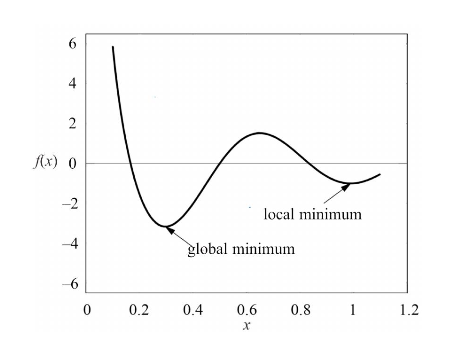
\includegraphics[width=0.5\textwidth]{imgs/notation_2}
		\caption{A local and a global minima of a function.}
	\end{figure}
	A \textcolor{red}{vector function}, denoted as $\mathrm{y}=\boldsymbol{f}(x)$ is a function that returns a vector $\mathrm{y}$. It can have a vector or a scalar argument.
\end{frame}

\subsection{Max and ArgMax}

\begin{frame}{Max and ArgMax}
	Given a set of values $\mathcal{A}=\left\{a_{1}, a_{2}, \ldots, a_{n}\right\}$,

	\begin{itemize}
		\item the operator $\max _{a \in \mathcal{A}} f(a)$ returns the highest value $f(a)$ for all elements in the set $\mathcal{A}$.
		\item the operator $\arg \max _{a \in \mathcal{A}} f(a)$ returns the element of the set $\mathcal{A}$ that maximizes $f(a)$.
	\end{itemize}
	Sometimes, when the set is implicit or infinite, we can write $\max _{a} f(a)$ or $\arg \max _{a} f(a)$. Operators min and arg min operate in a similar manner.

	\begin{tcolorbox}[enhanced jigsaw, breakable, pad at break*=1mm, colback=gray!20!white, colframe=black!85!black, title=\textbf{Example}]
		\begin{enumerate}
			\item \textbf{Set of Values} $\mathcal{A}$:$ \{ Alice: 12000, Bob: 15000, Charlie: 18000, Diana: 10000 \}$
			\item \textbf{Function} $f(a)$: This is the function mapping each salesperson to their sales figure. For instance, $f(Alice) = 12000$.
			\item \textbf{Using Max}: $\max_{a \in \mathcal{A}} f(a)$: This will return the highest sales figure, which is \$18,000.
			\item \textbf{Using Arg Max}: $\arg \max_{a \in \mathcal{A}} f(a)$: This will return the salesperson who achieved this highest sales figure, which is Charlie.
		\end{enumerate}
	\end{tcolorbox}
\end{frame}

\subsection{Assignment Operator}
\begin{frame}{Assignment Operator}
	The expression $a \leftarrow f(x)$ means that the variable $a$ gets the new value: the result of $f(x)$. We say that the variable $a$ gets assigned a new value.
	\begin{itemize}
		\item Similarly, $\mathbf{a} \leftarrow\left[a_{1}, a_{2}\right]$ means that the vector variable a gets the two-dimensional vector value $\left[a_{1}, a_{2}\right]$.
	\end{itemize}
\end{frame}

\subsection{Derivative and Gradient}
\begin{frame}{Derivative and Gradient}
	A \textbf{derivative} $f^{\prime}$ of a function $f$ is a function or a value that describes how fast $f$ grows (or decreases).
	\begin{itemize}
		\item If the derivative is a constant value, like 5 or -3 , then the function grows (or decreases) constantly at any point $x$ of its domain.
		\item If the derivative $f^{\prime}$ is a function, then the function $f$ can grow at a different pace in different regions of its domain.
		      \begin{itemize}
			      \item If the derivative $f^{\prime}$ is positive at some point $x$, then the function $f$ grows at this point.
			      \item If the derivative of $f$ is negative at some $x$, then the function decreases at this point. The derivative of zero at $x$ means that the function's slope at $x$ is horizontal.
		      \end{itemize}
	\end{itemize}
	The process of finding a derivative is called \textbf{differentiation}. Derivatives for basic functions are known. For example if $f(x)=x^{2}$, then $f^{\prime}(x)=2 x$; if $f(x)=2 x$ then $f^{\prime}(x)=2$; if $f(x)=2$ then $f^{\prime}(x)=0$ (the derivative of any function $f(x)=c$, where $c$ is a constant value, is zero).
\end{frame}

\begin{frame}
	If the function we want to differentiate is not basic, we can find its derivative using the \textbf{chain rule}.
	\begin{itemize}
		\item For instance if $F(x)=f(g(x))$, where $f$ and $g$ are some functions, then $F^{\prime}(x)=$ $f^{\prime}(g(x)) g^{\prime}(x)$.
		\item For example if $F(x)=(5 x+1)^{2}$ then $g(x)=5 x+1$ and $f(g(x))=(g(x))^{2}$. By applying the chain rule, we find $F^{\prime}(x)=2(5 x+1) g^{\prime}(x)=2(5 x+1) 5=50 x+10$.
	\end{itemize}
\end{frame}

\begin{frame}
	\textbf{Gradient} is the generalization of derivative for functions that take several inputs (or one input in the form of a vector or some other complex structure). A gradient of a function is a vector of \textbf{partial derivatives}.
	\begin{itemize}
		\item You can look at finding a partial derivative of a function as the process of finding the derivative by focusing on one of the function's inputs and by considering all other inputs as constant values.
	\end{itemize}

	The gradient of function $f$, denoted as $\nabla f$ is given by the vector $\left[\frac{\partial f}{\partial x^{(1)}}, \frac{\partial f}{\partial x^{(2)}}\right]$.
\end{frame}

\begin{frame}
	\textcolor{red}{For example,}
	\begin{itemize}
		\item if our function is defined as $f\left(\left[x^{(1)}, x^{(2)}\right]\right)=a x^{(1)}+b x^{(2)}+c$, then the partial derivative of function $f$ with respect to $x^{(1)}$, denoted as $\frac{\partial f}{\partial x^{(1)}}$, is given by,
		      $$
			      \frac{\partial f}{\partial x^{(1)}}=a+0+0=a
		      $$
		      where $a$ is the derivative of the function $a x^{(1)}$; the two zeroes are respectively derivatives of $b x^{(2)}$ and $c$, because $x^{(2)}$ is considered constant when we compute the derivative with respect to $x^{(1)}$, and the derivative of any constant is zero.
		\item Similarly, the partial derivative of function $f$ with respect to $x^{(2)}, \frac{\partial f}{\partial x^{(2)}}$, is given by,

		      $$
			      \frac{\partial f}{\partial x^{(2)}}=0+b+0=b \text {. }
		      $$
	\end{itemize}
\end{frame}

\section{Random Variable}
\begin{frame}{Random Variable}
	A \textbf{random variable}, usually written as an italic capital letter, like $X$, is a variable whose possible values are numerical outcomes of a random phenomenon.
	\begin{itemize}
		\item Examples of random phenomena with a numerical outcome include a toss of a coin (0 for heads and 1 for tails), a roll of a dice, or the height of the first stranger you meet outside. There are two types of random variables: \textbf{discrete} and \textbf{continuous}.
	\end{itemize}
	A \textbf{discrete random variable} takes on only a countable number of distinct values such as \textit{red,yellow,blue} or 1,2,3, ... .
\end{frame}

\begin{frame}
	The \textbf{probability distribution} of a discrete random variable is described by a list of probabilities associated with each of its possible values. This list of probabilities is called a \textbf{probability mass function} (pmf).
	\begin{itemize}
		\item For example: $\operatorname{Pr}(X=$ red $)=0.3, \operatorname{Pr}(X=$ yellow $)=0.45$, $\operatorname{Pr}(X=b l u e)=0.25$. Each probability in a probability mass function is a value greater than or equal to 0 . The sum of probabilities equals 1.
	\end{itemize}

	\begin{figure}
		\centering
		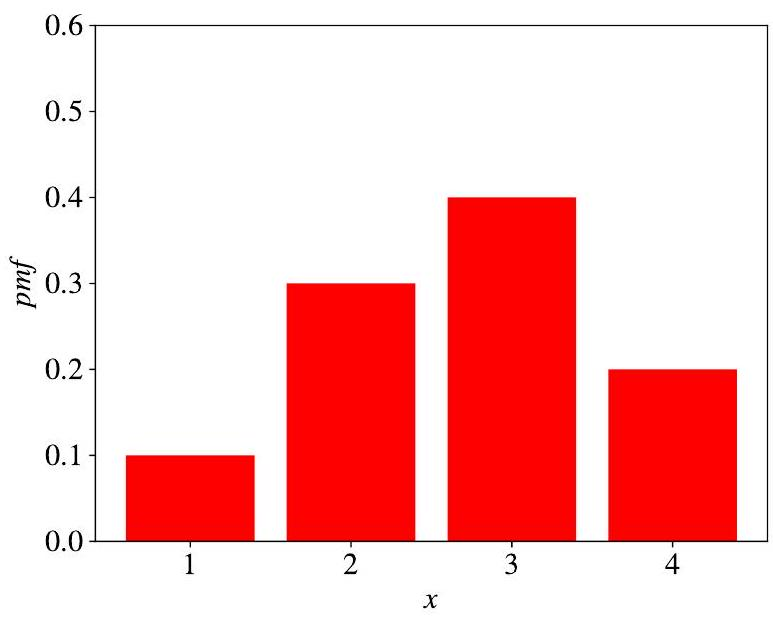
\includegraphics[width=0.4\textwidth]{imgs/notation_3.jpeg}
		\caption{A probability mass function}
	\end{figure}
\end{frame}

\begin{frame}
	A \textbf{continuous random variable} (CRV) takes an infinite number of possible values in some interval. Examples include height, weight, and time. Because the number of values of a continuous random variable $X$ is infinite, the probability $\operatorname{Pr}(X=c)$ for any $c$ is 0.
	\begin{itemize}
		\item Therefore, instead of the list of probabilities, the probability distribution of a CRV (a continuous probability distribution) is described by a \textbf{probability density function} (pdf). The pdf is a function whose codomain is nonnegative and the area under the curve is equal to 1.
	\end{itemize}
	\begin{figure}[ht]
		\centering
		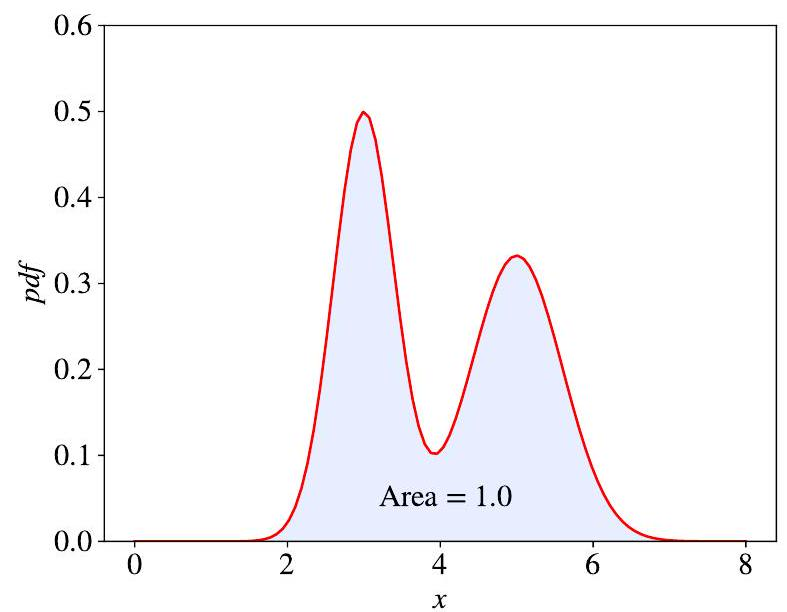
\includegraphics[width=0.4\linewidth]{imgs/notation_4.jpeg}
		\caption{A probability density function.}
	\end{figure}
\end{frame}

\begin{frame}
	Let a discrete random variable $X$ have $k$ possible values $\left\{x_{i}\right\}_{i=1}^{k}$. The \textbf{expectation} of $X$ denoted as $\mathbb{E}[X]$ is given by,

	$$
		\begin{aligned}
			\mathbb{E}[X] & \stackrel{\text { def }}{=} \sum_{i=1}^{k}\left[x_{i} \cdot \operatorname{Pr}\left(X=x_{i}\right)\right]                                                       \\
			              & =x_{1} \cdot \operatorname{Pr}\left(X=x_{1}\right)+x_{2} \cdot \operatorname{Pr}\left(X=x_{2}\right)+\cdots+x_{k} \cdot \operatorname{Pr}\left(X=x_{k}\right),
		\end{aligned}
	$$

	where $\operatorname{Pr}\left(X=x_{i}\right)$ is the probability that $X$ has the value $x_{i}$ according to the pmf. The expectation of a random variable is also called the \textbf{mean, average} or \textbf{expected} value and is frequently denoted with the letter $\mu$. \textcolor{red}{The expectation is one of the most important statistics of a random variable.}
\end{frame}

\begin{frame}
	The expectation of a continuous random variable $X$ is given by,

	$$
		\mathbb{E}[X] \stackrel{\text { def }}{=} \int_{\mathbb{R}} x f_{X}(x) d x
	$$

	where $f_{X}$ is the pdf of the variable $X$ and $\int_{\mathbb{R}}$ is the \textit{integral} of function $x f_{X}$.
	\begin{tcolorbox}[enhanced jigsaw, breakable, pad at break*=1mm, colback=gray!20!white, colframe=black!85!black, title=\textbf{Expectation for Continuous Random Variable}]
		\small
		For a continuous random variable \( X \) representing time in a coffee shop, uniformly distributed between 5 and 15 minutes, the probability density function (pdf) is \( f_X(x) = \frac{1}{10} \) for \( 5 \leq x \leq 15 \). The expected value \( \mathbb{E}[X] \) is calculated as follows:
		\begin{align*}
			\mathbb{E}[X] & = \int_{5}^{15} x \cdot \frac{1}{10} dx              \\
			              & = \frac{1}{10} \int_{5}^{15} x dx                    \\
			              & = \frac{1}{10} \left[ \frac{x^2}{2} \right]_{5}^{15} \\
			              & = 10 \text{ minutes}
		\end{align*}
	\end{tcolorbox}
\end{frame}

\begin{frame}
	Another important statistic is the \textbf{standard deviation}, defined as,

	$$
		\sigma \stackrel{\text { def }}{=} \sqrt{\mathbb{E}\left[(X-\mu)^{2}\right]}
	$$

	\textbf{Variance}, denoted as $\sigma^{2}$ or $\operatorname{var}(X)$, is defined as,

	$$
		\sigma^{2}=\mathbb{E}\left[(X-\mu)^{2}\right]
	$$

	For a discrete random variable, the standard deviation is given by:

	\[
		\sigma = \sqrt{\sum_{i=1}^{k} \operatorname{Pr}(X=x_i) (x_i - \mu)^2}
	\]


	where $\mu=\mathbb{E}[X]$.
\end{frame}

\begin{frame}
Integral is an equivalent of the summation over all values of the function when the function has a continuous domain.
\begin{itemize}
	\item  It equals the area under the curve of the function.
	\item  The property of the pdf that the area under its curve is 1 mathematically means that $\int_{\mathbb{R}} f_{X}(x) d x=1$.
\end{itemize}
Most of the time we don't know $f_{X}$, but we can observe some values of $X$. In machine learning, we call these values examples, and the collection of these examples is called a sample or a dataset.
\end{frame}

\section{Unbiased Estimators}
\begin{frame}{Unbiased Estimators}
	Because $f_{X}$ is usually unknown, but we have a sample $S_{X}=\left\{x_{i}\right\}_{i=1}^{N}$, we often content ourselves not with the true values of statistics of the probability distribution, such as expectation, but with their \textbf{unbiased estimators}.
	
	We say that $\hat{\theta}\left(S_{X}\right)$ is an unbiased estimator of some statistic $\theta$ calculated using a sample $S_{X}$ drawn from an unknown probability distribution if $\hat{\theta}\left(S_{X}\right)$ has the following property:
	
	$$
	\mathbb{E}\left[\hat{\theta}\left(S_{X}\right)\right]=\theta
	$$
	
	where $\hat{\theta}$ is a sample statistic, obtained using a sample $S_{X}$ and not the real statistic $\theta$ that can be obtained only knowing $X$; the expectation is taken over all possible samples drawn from $X$. Intuitively, this means that if you can have an unlimited number of such samples as $S_{X}$, and you compute some unbiased estimator, such as $\hat{\mu}$, using each sample, then the average of all these $\hat{\mu}$ equals the real statistic $\mu$ that you would get computed on $X$.
\end{frame}

\end{document}